\subsection{Compiled vs. Interpreted}
\begin{itemize}
	\item Language implementation can be compiled or interpreted.
	\begin{itemize}
	 	\item \textbf{Compiled}: program is converted into low-level machine code before execution.
	 	\item \textbf{Interpreted}: program is run step-by-step during execution.
	 \end{itemize} 
	 \begin{tabular}{l|l}
	 	Compiled & Interpreted \\
	 	\hline
	 	Faster & Slower (must go through execution engine) \\
	 	Less portable (needs recompile) & More portable \\
	 	Less flexible (complete at compile time) & More flexible 	 	
	 \end{tabular}

	 \item C++ is a compiled language, for this course we will use \textbf{g++} as our compiler
	 \item g++ wraps multiple steps:
	 \begin{enumerate}
	 	\item Preprocessing
	 	\item Compilation proper
	 	\item Assembly
	 	\item Linking
	 \end{enumerate}
\end{itemize}

\subsection{Preprocessing}
\begin{itemize}
	\item Expands all included libraries (e.g., \lstinline[style=C++]{#include, #define})
	\item To view what preprocessing does add the \lstinline[style=bash]{-E} flag, this will stop it after the preprocessing stage. (e.g., \lstinline[style=bash]{g++ -E hello.cpp -o hello.ii})
	\begin{center}
		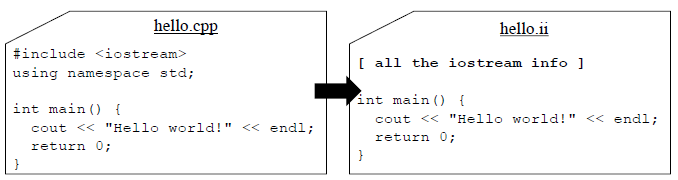
\includegraphics[scale=0.6]{sections/lec1/pre.png}
	\end{center}
\end{itemize}

\subsection{Compilation proper}
\begin{itemize}
	\item Converts C++ code into assembly instructions
	\item To view what compilation proper does add the \lstinline[style=bash]{-S} flag, this will stop it after the compilation proper stage. (e.g., \lstinline[style=bash]{g++ -S hello.ii -o hello.s})
	\begin{center}
		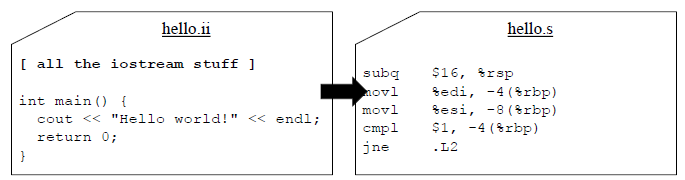
\includegraphics[scale=0.6]{sections/lec1/comp.png}
	\end{center}
\end{itemize}

\subsection{Assembly}
\begin{itemize}
	\item Converts assembly into binary
	\item Results in an \textbf{object file}
	\item To view what assembly does add the \lstinline[style=bash]{-c} flag, this will stop it after the assembly stage. (e.g., \lstinline[style=bash]{g++ -c hello.s -o hello.o})
	\begin{center}
		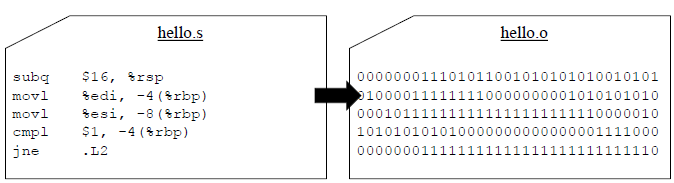
\includegraphics[scale=0.6]{sections/lec1/ass.png}
	\end{center}
\end{itemize}

\subsection{Linking}
\begin{itemize}
	\item Allows libraries and other object files to find each other
	\item Creates an executable
	\item \lstinline[style=bash]{g++ hello.o -o hello}
	\begin{center}
		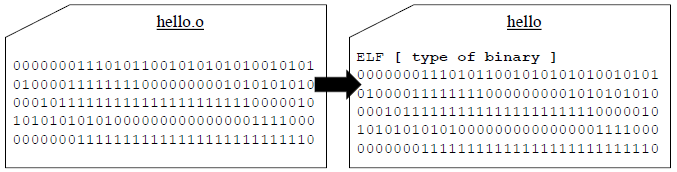
\includegraphics[scale=0.6]{sections/lec1/link.png}
	\end{center}
\end{itemize}

\subsection{Running the Executable}
\begin{enumerate}
	\item Type program call into shell (\lstinline[style=bash]{\% ./hello})
	\item Shell asks OS to run program
	\item OS loads executable into memory (disk$\to$RAM)
	\item OS begins execution
	\item Program executes and finishes
	\item Control transferred back to OS
\end{enumerate}